\documentclass[class=book, crop=false]{standalone}
\usepackage[subpreambles=true]{standalone}
\usepackage{import}
\usepackage{amsmath}
\usepackage{amssymb}
\usepackage[margin=1.2in]{geometry}
\usepackage[sorting = none,
            doi = true  %lesedato for url-adresse
            ]{biblatex} %none gir bibliografi i sitert rekkefølge
\addbibresource{reference.bib}
\usepackage{csquotes}


\begin{document}
%\chapter{Reinforcement learning}
\section{Intuitive introduction to reinforcement learning}
Reinforcement learning is an algorithm that learns through trial and error. The system consists of an agent that observes a state and responds to that by taking an action. Simply put, the agent will get a positive reward when it takes good actions and negative rewards for bad actions. When the agent takes a bad action, it will be less likely to chose that action again later. Similarly, when it gets a reward it will likely chose a similar action given the same observed state. By letting the agent see many states and explore different actions, it can eventually learn a policy that maximises expected future rewards. 

This algorithm is similar to how humans and animals learn. Imagine a dog seeing its owner holding a bag of treats. Obviously, the dog is keen on getting the treats, but is not sure what to do. The dog sees that the owner is putting his hand in front of its nose and yelling some command, but does not quit understand what to do. So it simply tries doing something. First, it might try to lean forward and smell the hand. Sadly, this does not result in any treat. Therefore, it continuous to try different actions, until it eventually happens to lift its front paw in the hand of the owner. At last, it receives a tasty treat from the owner. It has learned what action to take to get a treat. Next, the owner might rotate its arm in front of the dog. The dog might try to lift its front paw again, since that worked last time. Sadly, it does not get a reward this times. Therefore, it starts to explore new actions until it after some time tries to spin around. Again, it receives a treat. It has now learned that simply raising its front paw does not always result in a treat. It has to evaluate its observation before taking an action. 

The dog training is similar to an reinforcement learning algorithm. The dog is the agent that tries to figure own what actions to do, while the owner is the reward system. The advantage of the reinforcement algorithm is that it does not need a physical reward, and the agent can experiment much more quickly than a dog can. 

\section{Reinforcement algorithms}
Algorithms in machine learning and artificial intelligence are often divided into either supervised or unsupervised learning. Supervised learning is an algorithm using input data and labelled output data (target). The algorithm tries to map the input to the target in a manner that generalises well to unseen input data. Examples of supervised learning are regression and classification algorithms. Unsupervised learning is algorithms attempting to find structure in unlabelled data. Examples of such are clustering and anomaly detection. The terms \textit{supervised} and \textit{unsupervised} do not describe well the mechanisms of reinforcement learning algorithms. An reinforcement learning agent learns from interacting with an environment and receiving rewards based the action it takes. The agent's goal is not to use labelled data in some sense or explicitly finding general structures in the data. As a result, reinforcement learning is considered to be a category of its own\cite{Sutton1998}. 

\section{Markov decision process}\label{section:markov_decision_process}

A Markov decision process is a mathematical framework describing sequential decision making and interaction with an environment, where the outcome can be stochastic. This is precisely what
a general reinforcement algorithm attempts to do. The set of possible actions and states are respectively called the action space $\mathcal{A}$ and state space $\mathcal{S}$. For some reinforcement learning tasks, such as chess, the action space depends on the state $s$. For instance, it is not allowed to castle if an opponents piece is attacking some of the squares over which the king will move. In such cases, the action space $\mathcal{A}(s)$ is given by the state. The action space in an electric power system is dependent on the state, for instance if a power plant is out of operation. The environment starts at $t=0$ and is described by a state $s_{0} \in \mathcal{S}$. The agent preforms some action $a_{0}\in \mathcal{A}$ and receives a reward $r_{1}\in \mathcal{R} \subseteq \mathbb{R} $ based on how "good" that action is. The action $a_{0}$ interacts with the environment and gives a new state $s_{1}$. This starts the sequence of states, actions and rewards.


\begin{equation}
   \begin{aligned}\label{eq:theory:trajectory}
s_{0},a_{0},r_{1},s_{1}, a_{1},r_{2},s_{2},...
\end{aligned} 
\end{equation}

The interaction between the agent and environment is visualised in figure \ref{fig:theory:markov_decision_process} as a feedback loop.

\begin{figure}[ht!]
    \center
    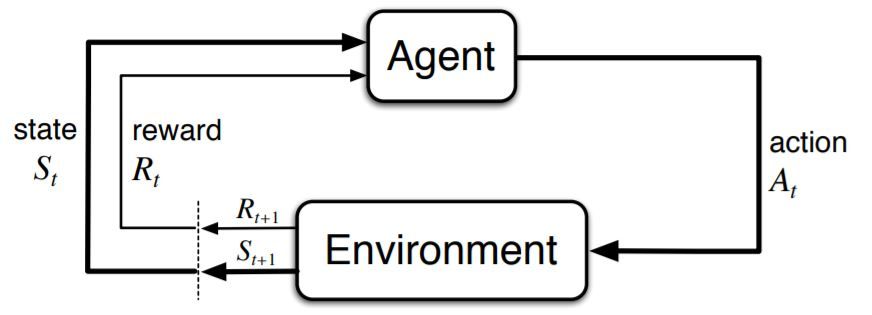
\includegraphics[height=3.5cm, width=10cm]{figures/markov_decision_processs.JPG}
    \caption[size = 9]{Interaction in a Markov decision process. Source: Sutton \cite{Sutton1998}}
    \label{fig:theory:markov_decision_process}
\end{figure}



The goal at each time step $t$ is to maximise the rewards in the future. How to formally define the reward maximising criterion depends on the nature of the task. Some tasks, such as playing a video game, are called episodic and have well-defined boundaries for start and end state. On the other hand, the electric power system is a continuous task that never should end if the agent does its job. For continuous tasks, let the discounted return $r^{\gamma}_{t}$ at time $t$ be defined as 


\begin{equation}
   \begin{aligned}\label{eq:theory:discounted_reward}
r^{\gamma}_{t} = r_{t+1} + \gamma r_{t+2} + \gamma^{2} r_{t+3} + ...
= \sum_{k=t}^{\infty} \gamma^{k-t}r_{k+1}
\end{aligned} 
\end{equation}
where $r_{t}$ is the reward received after action $a_{t}$ and $\gamma \in (0,1)$ is the discount factor. The goal of the agent at every time step $t$ could be to maximise the discounted return $r^{\gamma}_{t}$.



\section{Value and policy functions}

An agent selects actions in a given state is through its policy $\pi$. The policy of the agent decides what action to take in a given state by mapping the state space to the action space, $\pi: \mathcal{S} \to \mathcal{A}$. The policy can both be deterministic and stochastic. A deterministic policy maps a given state to the same action every time, while a stochastic policy maps the state to a probability distribution over the action space. For the deterministic case, the policy function $\pi$ is given by


\begin{equation}
   \begin{aligned}\label{eq:theory:policy_function_deterministic}
\pi(s) = a
\end{aligned} 
\end{equation}
where $a$ is the action chosen by the policy. Fot the stochastic case, it gives the probability of choosing action $a$.


\begin{equation}
   \begin{aligned}\label{eq:theory:policy_function_stochastic}
\pi(a|s) = \mathbb{P}(a|s)
\end{aligned} 
\end{equation}


The reinforcement algorithms used in this thesis are restricted to policy-gradient methods. These are methods that approximate the policy function using a neural network and updates its parameters using gradients. 

It is very convenient to able to evaluate a certain state before taking an action. $V^{\pi}$ is called the value function $V$ under the policy $\pi$ and gives a metric for the "value" of the current state. The reason for including "under the policy $\pi$" is that a state is valued differently depending on the policy used. For instance, the start position in chess will be evaluated better under the policy of a chess grand master, than under the policy of an amateur. The value function $V_{\pi}(s)$ is the expected discounted reward $r^{\gamma}_{t}$ as defined by \eqref{eq:theory:discounted_reward} given state $s$ and following the policy $\pi$.

\begin{equation}
   \begin{aligned}\label{eq:theory:value_function}
V_{\pi}(s) 
&= \mathbb{E}_{\pi}[r^{\gamma}_{t}| s=s_{t}]
\\
&= \mathbb{E}_{\pi}[ r_{t+1} + \gamma r_{t+2} + \gamma^{2} r_{t+3} + ...|s=s_{t}]
\end{aligned} 
\end{equation}

$Q_{\pi}(s,a)$ is called the action-value function, which quantifies the expected discounted return given the action $a_{t}$ in state $s_{t}$ and that the policy $\pi$ is followed thereafter. In other words, it can evaluate a specific action in a given state.  

\begin{equation}
   \begin{aligned}\label{eq:theory:action_value_function}
Q_{\pi}(s_{t},a_{t}) 
&= \mathbb{E}_{\pi}[r^{\gamma}_{t}|a=a_{t} ,s=s_{t}]
\\
&= \mathbb{E}_{\pi}[ r_{t+1} + \gamma r_{t+2} + \gamma^{2} r_{t+3} + ...|a=a_{t} ,s=s_{t}]
\end{aligned} 
\end{equation}




\section{Off-policy and on-policy}
A problem that arises when constructing a reinforcement learning algorithm is how to both be able to exploit a good policy and at the same time explore new policies. If an agent always follows its policy and picks the action it believes is the best, it will never explore new and perhaps better approaches to solve a problem. A solution to this problem is two have two different policies. One policy is called the target policy that is to be the optimal solution, while the other is called the behaviour policy and is for exploration of new behaviours\cite{Sutton1998}. A reinforcement learning algorithm using this approach is said to be learning off-policy.

\section{Deep deterministic policy gradient}
Silver et. al has developed an off-policy reinforcement algorithm called deep deterministic policy gradient (DDPG)\cite{pmlr-v32-silver14}. As the name suggest, the algorithm uses a deterministic approximation of the policy function instead of a stochastic version. The advantage with with a deterministic policy is that it does not have to integrate over action space in the search for the best policy. This section will outline the differences between stochastic and deterministic policy function. Both cases share similarities with each other. DDPG models the problem as a Markov decision problem as described in section \ref{section:markov_decision_process}.

The initial state distribution is described by $p_{1}(s_{1})$. There is a reward function $r: \mathcal{S} \times \mathcal{A} \to \mathcal{R} \subseteq \mathbb{R}$ and an action value function $Q^{\pi}:\mathcal{S} \times \mathcal{A} \to \mathbb{R}$ that evaluates an action $a$ in state $s$ under the policy $\pi$. The policy interacts with the environment by taking actions and generates a trajectory of states, action and rewards 
\begin{equation}
   \begin{aligned}\label{eq:theory:trajectory2}
h_{1:T} = s_{1},a_{1},r_{1},..., s_{T},a_{T},r_{T}
\end{aligned} 
\end{equation}
The objective function $J(\pi)$ that agent will maximise is the expected discounted return under the policy $\pi$

\begin{equation}
   \begin{aligned}\label{eq:theory:max_discounted_return}
J(\pi)
= \mathbb{E}_{\pi}[r^{\gamma}_{1}]
= \mathbb{E}_{\pi}[ r_{1} + \gamma r_{t+2} + \gamma^{2} r_{t+3} + ...]
\end{aligned} 
\end{equation}

\subsection{Stochastic policy approximation}\label{section:stochastic_policy_approx}
Consider a parametrised stochastic policy $\pi_{\theta}: \mathcal{S}\to \mathcal{P}(\mathcal{A})$ with parameters $\theta$ that maps the state space to a probability distribution over the action space. Let $p(s\to s',t,\pi)$ be the probability of transitioning from state $s$ to $s'$ in $t$ time steps. The discounted state distribution $\rho^{\pi}(s')$ is defined as   

\begin{equation}
   \begin{aligned}\label{eq:theory:discounted_state_distribution}
    \rho^{\pi}(s') = \int_{\mathcal{S}}\sum_{t=1}^{\infty }\gamma^{t-1}p_{1}(s)
    p(s \to s',t,\pi)ds
\end{aligned} 
\end{equation}
The performance objective can then be expressed as an expectation
\begin{equation}
   \begin{aligned}\label{eq:theory:objective_expected_stochastic}
    J(\pi_{\theta}) &= 
    \int_{\mathcal{S}}\rho^{\pi}(s) \int_{\mathcal{A}}\pi_{\theta}(a|s)r(a,s)da ds 
    \\
    &=
    \mathbb{E}_{s\sim \rho^{\pi},a \sim \pi_{\theta}}[r(s,a)]
\end{aligned} 
\end{equation}
 The way the agent learns is by computing the gradient of the objective with respect to the policy parameters $\theta$ and update the weights in that direction. The gradient of the stochastic policy is given is given by the policy gradient theorem (Sutton \cite{Sutton1998}) in equation \eqref{eq:theory:stochastic_gradient}.

\begin{equation}
   \begin{aligned}\label{eq:theory:stochastic_gradient}
    \nabla_{\theta} J(\pi_{\theta}) &= 
     \int_{\mathcal{S}}\rho^{\pi}(s)
     \int_{\mathcal{A}} \nabla_{\theta} \pi_{\theta}(a|s)Q^{\pi}(a,s)da ds
     \\
     &= \mathbb{E}_{s\sim \rho^{\pi},a \sim \pi_{\theta}}
     [\nabla_{\theta} \log \pi_{\theta}(a|s)Q^{\pi}(a,s) ]
\end{aligned} 
\end{equation}
Equation \eqref{eq:theory:stochastic_gradient} shows that the parameter update for the stochastic policy needs to integrates over the action space, which can be computationally costly.

\subsection{Deterministic policy approximation}
Consider a deterministic policy $\mu_{\theta}: \mathcal{S} \to \mathcal{A}$ with parameters $\theta$. Using the same definitions of discounted state distribution $\rho^{\mu}$ as in equation
\eqref{eq:theory:discounted_state_distribution}, the objective function is given as 

\begin{equation}
   \begin{aligned}\label{eq:theory:objective_expected_deterministic}
    J(\mu_{\theta}) =
    \int_{\mathcal{S}}
    \rho^{\mu}(s)r(s,\mu_{\theta}(s)) ds = \mathbb{E}_{s\sim \rho^{\mu}}[r(s,\mu_{\theta}(s))]
\end{aligned} 
\end{equation}
Silver et al \cite{pmlr-v32-silver14} proved that the deterministic policy gradient is given as 

\begin{equation}
   \begin{aligned}\label{eq:theory:objective_gradient_deterministic}
    \nabla_{\theta}J(\mu_{\theta}) &=
    \int_{\mathcal{S}}
    \rho^{\mu}(s)
    \nabla_{\theta} \mu_{\theta}(s)
    \nabla_{a} Q^{\mu}(s,a)|_{a = \mu_{\theta}(s)}ds 
    \\
    &= \mathbb{E}_{s\sim \rho^{\mu}}
    [    \nabla_{\theta} \mu_{\theta}(s)
    \nabla_{a} Q^{\mu}(s,a)|_{a = \mu_{\theta}(s)}]
\end{aligned} 
\end{equation}
In other words, it is the expectation of the matrix-vector product of the policy Jacobian matrix and the action-value gradient with respect to the actions under policy $\mu_{\theta}$. By convention, the columns of $\nabla_{\theta} \mu_{\theta}$ are the gradient of each action dimension. Silver et al argue that there are a class of function approximators that follow the gradient of the action-value function. Let $w$ be the parameters of the action-value approximator $Q^{w}(s,a)$ such that   

\begin{equation}
   \begin{aligned}\label{eq:theory:action-value_approx}
    Q^{\mu}(s,a,w) \approx Q^{\mu}(s,a)
\end{aligned} 
\end{equation}
and replace the action-value gradient $\nabla_{a} Q^{\mu}(s,a)$ in equation \eqref{eq:theory:objective_gradient_deterministic} by
the gradient of the approximation $\nabla_{a} Q^{\mu}(s,a,w)$

\subsection{Deterministic off-policy actor-critic}
Deep deterministic policy gradient is an off-policy learning algorithm. An off-policy algorithm has two different policies: a target policy $\mu_{\theta}(s)$ that is to be the final policy, and a stochastic behavioural policy $\beta(s,a)$ that is used for exploration to find different strategies. In other words, the target policy learns from the experiences of the behavioural policy. The off-policy objective performance in equation \eqref{eq:theory:objective_expected_deterministic} is altered by replacing the reward $r$ with the value function $V^{\mu}$ under the target policy $\mu$ and following the discounted state distribution of the behavioural policy $\rho^{\beta}$.

\begin{equation}
   \begin{aligned}\label{eq:theory:objective_expected_ooff_policy}
    J_{\beta}(\mu_{\theta}) &=
    \int_{\mathcal{S}}
    \rho^{\beta}(s)V^{\mu}(s) ds 
    \\
    &=
    \int_{\mathcal{S}}
    \rho^{\beta}(s)Q^{\mu}(s,\mu_{\theta}(s)) ds
\end{aligned} 
\end{equation}
The gradient of the modified objective is

\begin{equation}
   \begin{aligned}\label{eq:theory:objective_gradient_deterministic_off_policy}
    \nabla_{\theta}J_{\beta}(\mu_{\theta}) &\approx
    \int_{\mathcal{S}}
    \rho^{\beta}(s)
    \nabla_{\theta} \mu_{\theta}(s|a)
    Q^{\mu}(s,a)ds 
    \\
    &= \mathbb{E}_{s\sim \rho^{\beta}}
    [    \nabla_{\theta} \mu_{\theta}(s)
    \nabla_{a} Q^{\mu}(s,a)|_{a = \mu_{\theta}(s)}]
\end{aligned} 
\end{equation}

\subsection{Bellman equation}
There is a recursive relation between the action-value function in two consecutive states $s_{t}$ and $s_{t+1}$, known as the Bellman equation. Assume a deterministic policy $\mu_{\theta}$

\begin{equation}
   \begin{aligned}\label{eq:theory:bellman_equation}
Q^{\mu}(s_{t},a_{t}) 
&= \mathbb{E}_{r_{t},s_{t+1} \sim \mathcal{E}}
[r(s_{t},a_{t}) +\gamma Q^{\mu}(s_{t+1},\mu(s_{t+1}))]
\end{aligned} 
\end{equation}
This relation can be transformed into a loss function for the action-value function approximator $Q(s,a|\theta^{Q})$. Let the action value target $y_{t} $ be defined as 

\begin{equation}
   \begin{aligned}\label{eq:theory:action_value_target_bellman_equation}
y_{t} = r(s_{t},a_{t}) + \gamma Q(s_{t+1},\mu(s_{t+1})|\theta^{Q})
\end{aligned} 
\end{equation}
The action-value loss can be defined as 

\begin{equation}
   \begin{aligned}\label{eq:theory:action_value_loss_bellman_equation}
L(\theta^{Q}) 
&= \mathbb{E}_
{s_{t}\sim\rho^{\beta},a_{t} \sim \beta, r_{t} \sim \mathcal{E}}
[(Q^{\mu}(s_{t},a_{t})- y_{t})^{2}]
\end{aligned} 
\end{equation}
Notice that the expectation is in respect to the  state and action of the behavioural policy $\beta$. The loss should is zero if the action value approximator satisfies the bellman equation in \eqref{eq:theory:bellman_equation}.


\subsection{Experience replay and stability}
It has been proven difficult to use a naive implementation of the described DDPG algorithm with neural network as function approximators\cite{DBLP:journals/corr/LillicrapHPHETS15}. 




\end{document}

